\section{Mengenlehre}

\subsection{Definition Menge}

Eine Menge ist eine wohl bestimmte Zusammenfassung von Objekten.
Die Objekte heißen \emph{Elemente} der Menge.

\begin{description}[style=nextline]
	\item[\( x \in A \)] \( x \) ist Element der Menge \( A \)
	\item[\( x \notin A \)]  \( x \) ist nicht Element der Menge \( A \)
\end{description}

\subsection{Darstellungen}

\begin{description}[style=nextline]
	\item[Aufzählung]
	      \( A = \{ a, e, i, o, u \} \)
	\item[Beschreibung]
	      \( M = \{ x \mid x \text{ hat die Eigenschaft } E \} \)
	\item[Mengendiagramm]
	      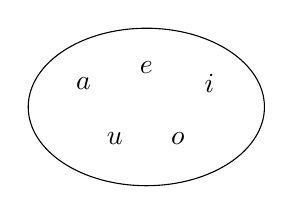
\begin{tikzpicture}
		      \draw[] (0,0) ellipse (1.5cm and 1cm);
		      \node[] at (-0.8, 0.3) {\( a \)};
		      \node[] at (0, 0.5) {\( e \)};
		      \node[] at (0.8, 0.3) {\( i \)};
		      \node[] at (0.4, -0.4) {\( o \)};
		      \node[] at (-0.4, -0.4) {\( u \)};
	      \end{tikzpicture}
\end{description}

\subsection{Beziehungen}

\begin{description}[style=nextline]
	\item[\( A = B \)]
	      \( A \) und \( B \) sind gleich, wenn sie dieselben Elemente enthalten.
	\item[\( A \subset B \)]
	      \( A \) ist echte Teilmenge von \( B \), wenn jedes Element von \( A \) auch
	      in \( B \) ist und \( A \) verschieden von \( B \) ist.
\end{description}


\subsection{Operationen}

{

	\def\circlea{(0,0) circle (1cm)}
	\def\circleb{(1.5,0cm) circle (1cm)}
	\def\universe{(0,0) circle (1.5cm)}

	\colorlet{circle edge}{mkblue}
	\colorlet{circle area}{mkblue!20}

	\tikzset{
		filled/.style={fill=circle area, draw=circle edge, thick},
		outline/.style={draw=circle edge, thick}
	}

	\def\vennaandb{\begin{tikzpicture}
			\begin{scope}
				\clip \circlea;
				\fill[filled] \circleb;
			\end{scope}
			\draw[outline] \circlea node {\( A \)};
			\draw[outline] \circleb node {\( B \)};
		\end{tikzpicture}
	}

	\def\vennaorb{
		\begin{tikzpicture}
			\draw[filled] \circlea node {\( A \)}
			\circleb node {\( B \)};
			\draw[outline] \circlea node {\( A \)};
			\draw[outline] \circleb node {\( B \)};
		\end{tikzpicture}
	}

	\def\vennaminusb{
		\begin{tikzpicture}
			\begin{scope}
				\clip \circlea;
				\draw[filled, even odd rule] \circlea node {\( A \)}
				\circleb;
			\end{scope}
			\draw[outline] \circlea node {\( A \)};
			\draw[outline] \circleb node {\( B \)};
		\end{tikzpicture}
	}

	\def\vennnota{
		\begin{tikzpicture}
			\begin{scope}
				\clip \universe;
				\draw[filled, even odd rule, above left] \universe node {} \circlea;
			\end{scope}
			\draw[outline] \circlea node {\( A \)};
		\end{tikzpicture}
	}

	\begin{tabular}{c m{5cm} m{4cm}}
		\( A \cap B \)      & \textbf{Schnittmenge} von \( A \) und \( B \) & \vennaandb   \\
		\( A \cup B \)      & \textbf{Vereinigung} von \( A \) und \( B \)  & \vennaorb    \\
		\( A \setminus B \) & \textbf{Differenz}, \( A \) ohne \( B \)      & \vennaminusb \\
		\(\bar{A}\)         & \textbf{Komplement} von \(A \)                & \vennnota
	\end{tabular}

}
